\documentclass{presentation}

\title{Συναρτήσεις} 
\subtitle{Μετατοπίσεις Συναρτήσεων}
\author[Λόλας]{Κωνσταντίνος Λόλας }


\begin{document}

\begin{frame}
  \titlepage\end{frame}

\begin{frame}{Στόχοι του μαθήματος}
  \begin{itemize}[<+->]
    \item Να μετατοπίζουμε τη γραφική παράσταση μιας οποιασδήποτε συνάρτησης.
    \item Να αναγνωρίζουμε μετατοπίσεις προς τα πάνω, κάτω, αριστερά και δεξιά.
    \item Να συνδέουμε τον τύπο της συνάρτησης με τη μετατόπιση της γραφικής της παράστασης.
  \end{itemize}
\end{frame}

\begin{frame}{Πώς φέρνω βόλτα την συνάρτηση}
  \begin{itemize}[<+->]
    \item Πάνω - Κάτω
    \item Αριστερά - Δεξιά
    \item Συμμετρικά ως προς $x$-άξονα
    \item Συμμετρικά ως προς $y$-άξονα
    \item Ξεχείλωμα
    \item Συμπίεση...
  \end{itemize}
\end{frame}

\begin{frame}{Τι κάνει το $f(x)+c$;}
  Το $f(x)$ είναι το $y$ άρα...

  \begin{itemize}[<+->]
    \item<2-> Αν $c>0$, η γραφική παράσταση μετατοπίζεται προς τα πάνω κατά $c$ μονάδες.
    \item<3-> Αν $c<0$, μετατοπίζεται προς τα κάτω κατά $|c|$ μονάδες.
    \item<4-> Αν $c=0$, παραμένει αμετάβλητη.
  \end{itemize}
\end{frame}

\begin{frame}{Τι κάνει το $f(x-c)$;}
  Το $c$ επηρεάζει τα $x$ άρα...

  \begin{itemize}[<+->]
    \item<2-> Αν $c>0$, η γραφική παράσταση μετατοπίζεται προς τα δεξιά κατά $c$ μονάδες.
    \item<3-> Αν $c<0$, μετατοπίζεται προς τα αριστερά κατά $|c|$ μονάδες.
    \item<4-> Αν $c=0$, παραμένει αμετάβλητη.
  \end{itemize}
\end{frame}

\begin{frame}{Τι κάνει το $-f(x)$;}
  Το $-$ αλλάζει το πρόσημο του $y$ άρα...

  \begin{itemize}[<+->]
    \item<2-> Τα θετικά $y$ γίνονται αρνητικά
    \item<3-> Τα αρνητικά $y$ γίνονται θετικά...
  \end{itemize}
\end{frame}

\begin{frame}{Τι κάνει το $f(-x)$;}
  Το $-$ αλλάζει το πρόσημο του $x$ άρα...

  \begin{itemize}[<+->]
    \item<2-> Τα θετικά $x$ γίνονται αρνητικά
    \item<3-> Τα αρνητικά $x$ γίνονται θετικά...
  \end{itemize}
\end{frame}

\begin{frame}{Τι κάνει το $|f(x)|$;}
  Το $| \cdot |$ παίρνει την απόλυτη τιμή του $y$ άρα...

  \begin{itemize}[<+->]
    \item<2-> Τα θετικά $y$ παραμένουν θετικά
    \item<3-> Τα αρνητικά $y$ γίνονται θετικά...
  \end{itemize}
\end{frame}

\begin{frame}{Τι κάνει το $a f(x)$;}
  Το $a$ πολλαπλασιάζει το $y$ άρα...

  \begin{itemize}[<+->]
    \item<2-> Αν $|a|>1$, η γραφική παράσταση "ξεχειλώνει" κατακόρυφα.
    \item<3-> Αν $0<|a|<1$, η γραφική παράσταση "συμπιέζεται" κατακόρυφα.
    \item<4-> Αν $a<0$?
  \end{itemize}
\end{frame}

\begin{frame}{Τι κάνει το $f(a x)$;}
  Το $a$ επηρεάζει τα $x$ άρα...

  \begin{itemize}[<+->]
    \item<2-> Αν $|a|>1$, η γραφική παράσταση "συμπιέζεται" οριζόντια.
    \item<3-> Αν $0<|a|<1$, η γραφική παράσταση "ξεχειλώνει" οριζόντια.
    \item<4-> Αν $a<0$?
  \end{itemize}
\end{frame}

\begin{frame}{Συμπέρασμα}
  Οι μετατοπίσεις και οι αλλαγές κλίμακας των συναρτήσεων μπορούν να κατανοηθούν με βάση το πώς επηρεάζουν τα $x$ και $y$.

  \begin{itemize}[<+->]
    \item Μετατοπίσεις πάνω/κάτω: $f(x) + c$
    \item Μετατοπίσεις αριστερά/δεξιά: $f(x - c)$
    \item Αντιστροφή ως προς $x$-άξονα: $-f(x)$
    \item Αντιστροφή ως προς $y$-άξονα: $f(-x)$
    \item Απόλυτη τιμή: $|f(x)|$
    \item Κατακόρυφη κλίμακα: $a f(x)$
    \item Οριζόντια κλίμακα: $f(a x)$
  \end{itemize}
\end{frame}

\exercises

\begin{askisi}
  Αφού σχεδιάσετε την συνάρτηση $f(x)=|x|$, να σχεδιάσετε στο ίδιο σύστημα αξόνων τις συναρτήσεις:
  \begin{itemize}
    \item $|x-2|$
    \item $|x|+3$
    \item $-|x+2|+1$
  \end{itemize}
\end{askisi}

\begin{askisi}
  Δίνεται η συνάρτηση $f(x)=x^2+4x+3$.
  \begin{itemize}
    \item Να βρείτε τα $α$ και $β$ ώστε $f(x)=(x+α)^2+β$
    \item Να σχεδιάσετε τη γραφική παράσταση της συνάρτησης $f(x)$
  \end{itemize}
\end{askisi}

\begin{askisi}
  Αν η συνάρτηση $f(x)$ είναι η γκρι γραμμή στο διπλανό σχήμα, να βρείτε τον τύπο της συνάρτησης που σχηματίζει η πορτοκαλί γραμμή, γνωρίζοντας ότι προκύπτει από την $f$ με μετατοπίσεις και αλλαγές κλίμακας.

  \begin{figure}
    \centering
    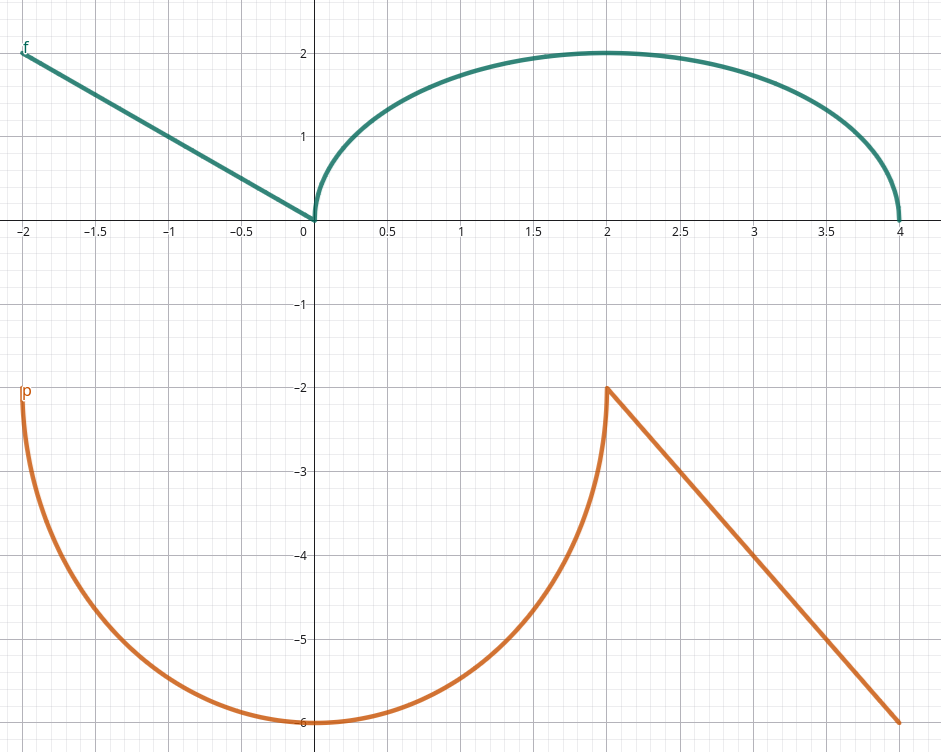
\includegraphics[width=0.6\textwidth]{./images/metatop.png}
  \end{figure}
\end{askisi}

\end{document}